\chapter{Длинные струны и соответствие со чёрной дырой}

\lectureoverview{Чёрная дыра обладает энтропией, значит, у неё должны быть микроскопические степени свободы. Мы построим простейшее струнно-теоретическое описание этих степеней свободы: сначала подсчитаем состояния длинной возбуждённой струны, затем будем изменять струнную константу связи, пока струнное описание и описание чёрной дыры не сойдутся. Окончательное равенство намеренно оставлено как задачу, которую нужно завершить на следующей лекции.}

\section{Энтропия требует микроскопических носителей}

Сказать, что система имеет большую энтропию, значит сказать, что она может скрывать большой объём микроскопической информации. Ванна с горячей водой может иметь энтропию порядка \(10^{30}\). Уже это утверждение говорит нам, что имеется чрезвычайно много микроскопических степеней свободы, независимо от того, захотим ли мы рассматривать их по молекулам. Термодинамика может определить энтропию, измеряя энергию и температуру, но она не указывает, какие объекты её несут.

Гидродинамика делает это различие привычным. Она описывает плотность, скорость, давление и макроскопическое течение, не обращаясь к атомам. Если добавить термодинамику, то обнаруживается, что такая среда обладает энтропией. Энтропия указывает на микроскопическую структуру, которую огрублённые уравнения не показывают; она ставит новый вопрос, а не отвечает на него.

Чёрные дыры ставят ту же задачу, но в более острой форме. Предложение Бекенштейна, завершённое вычислением Хокинга, приписывает энтропию, пропорциональную площади горизонта. Общая теория относительности определяет геометрию и её термодинамику, но не даёт перечня микроскопических состояний. Что это за малые, многочисленные объекты, конфигурации которых объясняют закон площади? В теории струн есть конкретный кандидат. Развиваемый здесь аргумент намеренно качественный: он правильно воспроизводит параметрическую зависимость, опуская численные константы и формальный аппарат полного подсчёта состояний.

\section{Три масштаба и одна ловушка в обозначениях}

Гравитация задаёт выделенную длину — планковскую длину,
\begin{equation}
\ell_p=\sqrt{\frac{G_N\hbar}{c^3}}.
\label{eq:l06-planck-si}
\end{equation}

\begin{classroomqa}
\audiencequestion{Какая комбинация \(G_N\), \(\hbar\) и \(c\) даёт планковскую длину?\lecturetimestamp{00:06:08}}
\lecturerresponse{Это \(\sqrt{G_N\hbar/c^3}\), примерно \(10^{-33}\) сантиметров. Мы сразу положим \(\hbar=c=1\), и тогда соотношение станет гораздо проще.}
\end{classroomqa}

В естественных единицах,
\begin{equation}
\hbar=c=1,
\qquad
G_N=\ell_p^2.
\label{eq:l06-planck-area}
\end{equation}
Следовательно, постоянная Ньютона имеет размерность площади. Поэтому площадь, делённая на \(G_N\), безразмерна и может быть энтропией.

В теории струн есть вторая длина, \(\ell_s\). Нагрейте струну или переведите её в сильно возбуждённое состояние, и она будет колебаться на многих масштабах. В этой элементарной картине характерный наименьший масштаб — длина струны. Можно рассматривать \(\ell_s\) как размер, связанный с одной элементарной единицей колебания струны.

Третья величина — безразмерная струнная константа связи \(g_s\). Она управляет расщеплением и слиянием: струна может разделиться на две струны, или возбуждённая струна может испустить квант замкнутой струны.

\begin{classroomqa}
\audiencequestion{Каков физический смысл струнной константы связи?\lecturetimestamp{00:09:20}}
\lecturerresponse{Она определяет вероятность струнного взаимодействия, например расщепления, когда струна пересекает саму себя. Точнее, \(g_s\) — это амплитуда взаимодействия; соответствующая вероятность или скорость начинается с члена порядка \(g_s^2\).}
\end{classroomqa}

Испущенное безмассовое возбуждение замкнутой струны может быть гравитоном. В этом отношении \(g_s\) играет роль, аналогичную электрическому заряду: это множитель, приписанный вершине взаимодействия.\editorialnote{В лекции \(g_s\) попеременно называется вероятностью и амплитудой. В теории возмущений это константа связи на уровне амплитуды; вероятности и скорости содержат её квадрат.}

\section{Почему в гравитации фигурирует \texorpdfstring{\(g_s^2\)}{the Coupling Squared}}

Рассмотрим сначала картину обмена в электромагнетизме. Один заряженный объект испускает фотон с фактором \(e\), а второй поглощает его с ещё одним фактором \(e\). Поэтому амплитуда обмена содержит \(e^2\). Эта картина не означает, что здесь буквально летит классический снаряд, но она правильно показывает, как входит константа связи.

\begin{figure}[htbp]
\centering
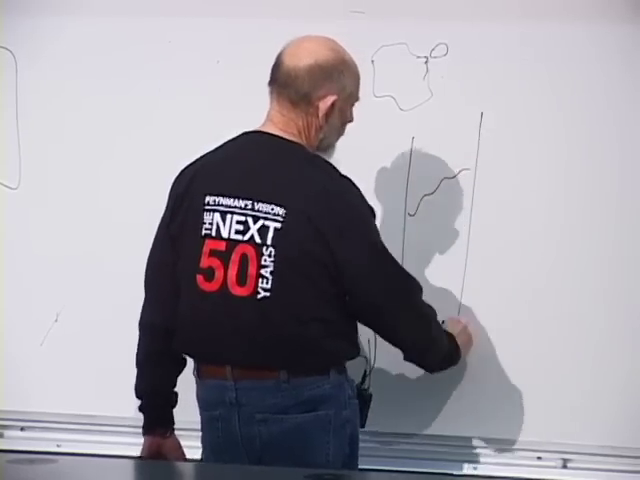
\includegraphics[width=0.72\textwidth]{lecture_06_figure_03.png}
\caption{Завершённые на доске схемы обмена: константа связи приписывается при испускании и ещё раз при поглощении.}
\lectureframe{00:11:30.000}
\end{figure}

В струнно-теоретической версии фотон заменяется гравитоном, а электрический заряд — на \(g_s\). Один фактор сопровождает испускание, а другой — поглощение, так что сила гравитационного взаимодействия масштабируется как \(g_s^2\).

На больших расстояниях то же взаимодействие должно воспроизводить закон тяготения Ньютона,
\begin{equation}
F_{\mathrm{grav}}\sim G_N\frac{M_1M_2}{r^2}.
\end{equation}
Массы и обратноквадратичная зависимость описывают источники и распространение; здесь нам важен множитель связи, который их умножает.

\begin{figure}[htbp]
\centering
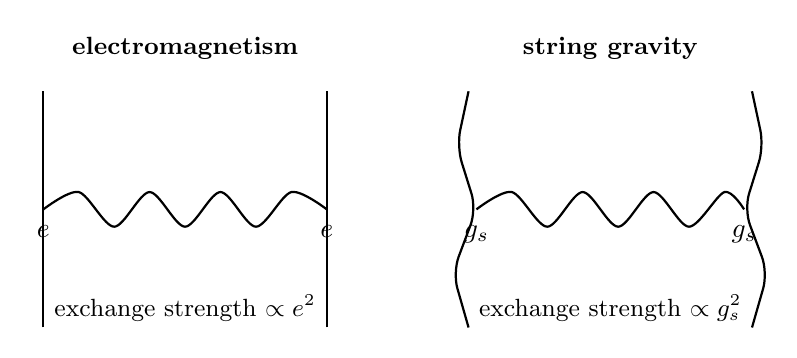
\begin{tikzpicture}[x=1cm,y=1cm]
  \node[font=\small\bfseries] at (1.8,3.55) {electromagnetism};
  \draw[line width=0.8pt] (0,0) -- (0,3);
  \draw[line width=0.8pt] (3.6,0) -- (3.6,3);
  \draw[line width=0.8pt] plot[smooth] coordinates {(0,1.5) (0.45,1.72) (0.9,1.28) (1.35,1.72) (1.8,1.28) (2.25,1.72) (2.7,1.28) (3.15,1.72) (3.6,1.5)};
  \node[below] at (0,1.42) {\(e\)};
  \node[below] at (3.6,1.42) {\(e\)};
  \node[font=\small] at (1.8,0.25) {exchange strength \(\propto e^2\)};
  \node[font=\small\bfseries] at (7.2,3.55) {string gravity};
  \draw[line width=0.8pt,rounded corners=6pt] (5.4,0) -- (5.2,0.7) -- (5.5,1.5) -- (5.25,2.3) -- (5.4,3);
  \draw[line width=0.8pt,rounded corners=6pt] (9,0) -- (9.2,0.7) -- (8.9,1.5) -- (9.15,2.3) -- (9,3);
  \draw[line width=0.8pt] plot[smooth] coordinates {(5.5,1.5) (5.95,1.72) (6.4,1.28) (6.85,1.72) (7.3,1.28) (7.75,1.72) (8.2,1.28) (8.65,1.72) (8.9,1.5)};
  \node[below] at (5.5,1.42) {\(g_s\)};
  \node[below] at (8.9,1.42) {\(g_s\)};
  \node[font=\small] at (7.2,0.25) {exchange strength \(\propto g_s^2\)};
\end{tikzpicture}
\caption{Аналогия для подсчёта степеней константы связи. Каждый конец обмениваемого кванта даёт по одному фактору взаимодействия.}
\end{figure}

Это наблюдение почти определяет постоянную Ньютона. Константа связи \(g_s\) безразмерна, тогда как в четырёх измерениях \(G_N\) имеет размерность квадрата длины. Доступная микроскопическая длина — \(\ell_s\), поэтому
\begin{equation}
G_N\sim g_s^2\ell_s^2.
\label{eq:l06-newton-string}
\end{equation}
Объединяя это с уравнением~\eqref{eq:l06-planck-area}, получаем
\begin{equation}
\ell_p\sim g_s\ell_s.
\label{eq:l06-planck-string}
\end{equation}

\begin{figure}[htbp]
\centering
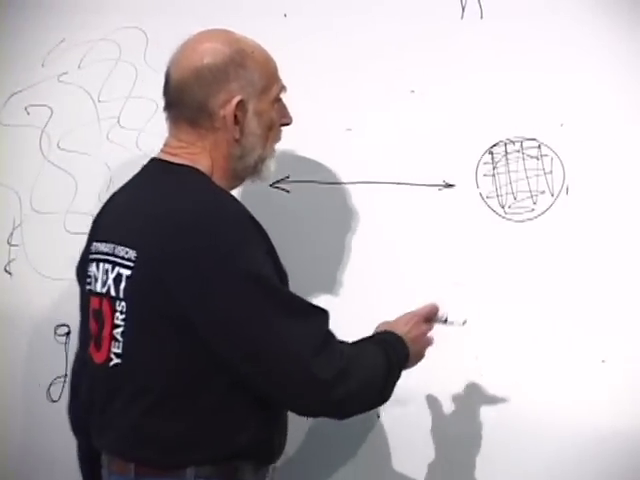
\includegraphics[width=0.72\textwidth]{lecture_06_figure_04.png}
\caption{Основные соотношения, оставленные на доске: \(\ell_p^2=G_N\) и \(\ell_p\sim g_s\ell_s\).}
\lectureframe{00:15:45.000}
\end{figure}

Уравнение~\eqref{eq:l06-newton-string} — это упрощённое соотношение, используемое на протяжении всей этой лекции.\editorialnote{В компактифицированной теории струн эффективная четырёхмерная постоянная Ньютона зависит также от объёма компактификации и от конвенций с коэффициентами порядка единицы. В лекции эти данные опускаются, чтобы выделить масштабирование соответствия.}

\begin{classroomqa}
\audiencequestion{Является ли \(g_s\) больше или меньше единицы, и какая длина больше?\lecturetimestamp{00:16:00}}
\lecturerresponse{Мы работаем при слабой связи, \(g_s<1\). Тогда из \(\ell_p\sim g_s\ell_s\) следует, что длина струны больше планковской длины. Сильная связь требует другого описания и здесь не нужна.}
\end{classroomqa}

\section{Подсчёт для чёрной дыры}

Опуская постоянную Больцмана и численные множители, энтропия Бекенштейна--Хокинга равна
\begin{equation}
S_{\mathrm{BH}}=\frac{A}{4G_N}sim\frac{A}{G_N}sim\frac{A}{\ell_p^2}.
\label{eq:l06-bh-area}
\end{equation}
Множитель \(1/4\) точен в полуклассической формуле, но в этом аргументе на уровне масштабирования он не играет роли.

\begin{classroomqa}
\audiencequestion{Указывает ли индекс ``BH'' на чёрную дыру или на Бекенштейна--Хокинга?\lecturetimestamp{00:16:51}}
\lecturerresponse{Для наших целей он может напоминать и об одном, и о другом. Важно то, что энтропия — это площадь горизонта, измеренная в единицах планковской площади.}
\end{classroomqa}

Для четырёхмерной чёрной дыры Шварцшильда,
\begin{equation}
R_s=2G_NM,
\qquad
A=4\pi R_s^2.
\end{equation}
Отбрасывая \(2\) и \(4\pi\), как это делается в лекции,
\begin{align}
S_{\mathrm{BH}}
&\sim \frac{R_s^2}{G_N}
\sim \frac{(G_NM)^2}{G_N} \\
&\sim M^2G_N
\sim M^2\ell_p^2.
\label{eq:l06-bh-mass}
\end{align}
Именно эту форму мы будем сравнивать со струнным подсчётом.

\section{Длинная струна как случайное блуждание}

Начнём с маленькой струны и будем закачивать в неё энергию. Типичная сильно возбуждённая струна не остаётся аккуратной петлёй. Она превращается в длинный запутанный объект, как леска на безнадёжно запутавшейся катушке. У этой путаницы есть энтропия, потому что огромное число конфигураций макроскопически выглядит одинаково.

Чтобы их подсчитать, заменим пространство решёткой, рёбра которой имеют длину \(\ell_s\). Узлы — это вершины, рёбра — линии, а элементарные квадраты — плакеты. Струна представляется связной последовательностью рёбер. Эта модель намеренно груба, но её экспоненциальный подсчёт состояний воспроизводит нужное масштабирование.

\begin{figure}[htbp]
\centering
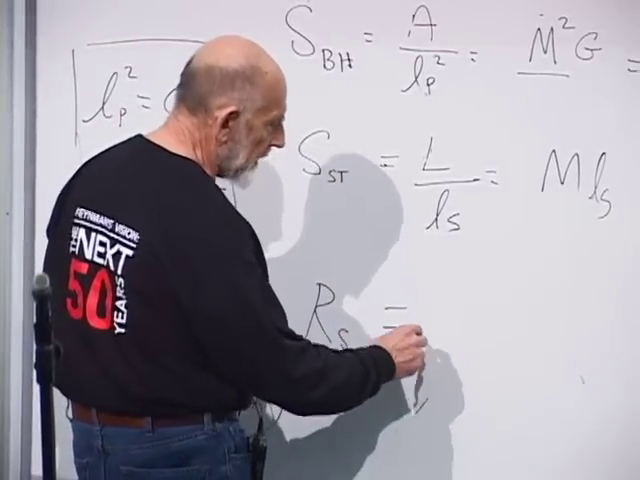
\includegraphics[width=0.72\textwidth]{lecture_06_figure_05.png}
\caption{Двумерная решёточная модель. Синий отрезок отмечает один шаг струны; в каждом узле учитываются все четыре возможных продолжения.}
\lectureframe{00:23:50.000}
\end{figure}

\begin{classroomqa}
\audiencequestion{Сколько вариантов есть на каждом шаге этого модельного блуждания?\lecturetimestamp{00:22:43}}
\lecturerresponse{Четыре на квадратной решётке, поскольку немедленный шаг назад разрешён. В трёх измерениях их было бы шесть. Другая решётка изменит конкретное число, но не тот факт, что число блужданий растёт экспоненциально с числом рёбер.}
\end{classroomqa}

Если у струны \(n\) рёбер, то двумерный модельный подсчёт даёт
\begin{equation}
\Omega_n\sim4^n.
\label{eq:l06-walk-count}
\end{equation}
Есть один исключительный прямой путь, но это лишь одно состояние среди \(4^n\). Типичный путь многократно складывается и образует запутанный клубок. При больших \(n\) почти каждая случайно сгенерированная конфигурация качественно похожа на любую другую.

Энтропия — это логарифм числа макроскопически неразличимых конфигураций:
\begin{equation}
S_{\mathrm{st}}=\log\Omega_n\sim n\log4\sim n.
\label{eq:l06-string-entropy-n}
\end{equation}

\begin{classroomqa}
\audiencequestion{Почему энтропия оказывается пропорциональной \(n\), а не \(4^n\)?\lecturetimestamp{00:25:39}}
\lecturerresponse{Энтропия есть логарифм числа состояний. Поэтому \(\log(4^n)=n\log4\), а множитель \(\log4\) — это константа порядка единицы, которую мы опустим.}
\end{classroomqa}

Если \(L\) — это контурная длина, получаемая, если проследить струну от одного конца до другого, то
\begin{equation}
n=\frac{L}{\ell_s},
\qquad
S_{\mathrm{st}}\sim\frac{L}{\ell_s}.
\label{eq:l06-string-entropy-length}
\end{equation}
Здесь \(L\) — не диаметр спутанного клубка. Это значительно большее расстояние, измеряемое вдоль струны.

Теперь перейдём от контурной длины к массе. При \(c=\hbar=1\) масса имеет размерность обратной длины. Поэтому одно звено размера струны имеет массу порядка
\begin{equation}
m_{\mathrm{link}}\sim\frac{1}{\ell_s}.
\label{eq:l06-link-mass}
\end{equation}

\begin{classroomqa}
\audiencequestion{Почему масса одного звена должна масштабироваться как \(1/\ell_s\)?\lecturetimestamp{00:29:20}}
\lecturerresponse{В этих единицах масса имеет размерность обратной длины, и \(\ell_s\) — единственная доступная длина. Эквивалентно, натяжение струны порядка \(1/\ell_s^2\), умноженное на длину звена \(\ell_s\), даёт тот же результат.}
\end{classroomqa}

Тогда для полной струны имеем
\begin{equation}
M\sim n m_{\mathrm{link}}
\sim\frac{n}{\ell_s}
\sim\frac{L}{\ell_s^2},
\qquad
L\sim M\ell_s^2.
\label{eq:l06-string-mass}
\end{equation}
Подстановка в уравнение~\eqref{eq:l06-string-entropy-length} даёт
\begin{equation}
S_{\mathrm{st}}\sim M\ell_s.
\label{eq:l06-string-entropy-mass}
\end{equation}
Решёточное случайное блуждание не учитывает ограничений мирового листа и численных коэффициентов, но экспоненциальный рост спектра сильно возбуждённой струны даёт то же ведущее масштабирование.\editorialnote{Конструкция со случайным блужданием — это мнемоника для плотности струнных состояний на высоких уровнях, а не буквальная дискретизация фундаментальной струны.}

\section{Несовпадение, с которого начинается аргумент}

Теперь имеются два ответа
\begin{equation}
S_{\mathrm{BH}}\sim M^2\ell_p^2,
\qquad
S_{\mathrm{st}}\sim M\ell_s.
\label{eq:l06-two-entropies}
\end{equation}
Они похожи друг на друга, но при фиксированной массе и произвольной константе связи не равны. Выражение для чёрной дыры квадратично по \(M\); струнное выражение линейно. Нельзя просто объявить горячую струну чёрной дырой, не объяснив, как встречаются эти два режима.

\begin{figure}[htbp]
\centering
\includegraphics[width=0.78\textwidth]{lecture_06_figure_06.png}
\caption{Сопоставление на доске в чистом виде: энтропия чёрной дыры сверху, энтропия длинной струны снизу, а слева сохранены соотношения Планка--струны.}
\lectureframe{00:33:20.000}
\end{figure}

На этом лекция прервалась. Эта пауза полезна: несовпадение — не провал идеи, а указание на то, что нужно сравнивать одно и то же состояние, меняя силу гравитации.

\section{Поворачивая ручку константы связи}

Будем держать \(\ell_s\) фиксированной и представим, что \(g_s\) можно менять. При \(g_s=0\) струны не расщепляются и не сливаются, а гравитация исчезает, поскольку \(G_N\sim g_s^2\ell_s^2\). Тогда состояние с достаточно большой энергией представляет собой длинную слабо взаимодействующую струну.

Медленно увеличим \(g_s\). Струнные взаимодействия становятся возможными и, что важнее для данного рассуждения, гравитация усиливается.

\begin{classroomqa}
\audiencequestion{По мере увеличения \(g_s\) не состоит ли первый эффект просто в том, что струна распадается на более короткие струны?\lecturetimestamp{00:36:29}}
\lecturerresponse{Расщепление и слияние становятся возможными, но держите \(\ell_s\) фиксированной и прослеживайте состояние с высокой энтропией. Главный эффект состоит в том, что растёт \(G_N\), так что собственная гравитация длинной струны стягивает спутанный клубок внутрь.}
\end{classroomqa}

Объект сжимается и становится плотнее. Его гравитационная потенциальная энергия отрицательна, так что сжатие уменьшает его полную энергию и тем самым массу.

\begin{classroomqa}
\audiencequestion{Увеличивается или уменьшается энергия, когда собственная гравитация стягивает струну?\lecturetimestamp{00:37:48}}
\lecturerresponse{Она уменьшается. Энергия связи становится более отрицательной. Масса вдоль этого пути не обязана оставаться фиксированной, хотя мы продолжаем отслеживать то же самое состояние.}
\end{classroomqa}

В конце концов размер объекта становится сравнимым с его радиусом Шварцшильда. После этого естественным становится описание как чёрной дыры. Более сильное начальное возбуждение достигает этого условия при меньшей связи, потому что более массивному объекту нужна меньшая сила гравитации, чтобы образовать горизонт.

\begin{figure}[htbp]
\centering
\resizebox{0.95\linewidth}{!}{%
\begin{tikzpicture}[x=1cm,y=1cm,>=Latex]
  \draw[->,line width=0.9pt] (0,0) -- (11,0) node[right] {increasing \(g_s\)};
  \node[draw,rounded corners,align=center,minimum width=2.6cm,minimum height=1.15cm] at (1.8,1.5) {long excited string\\weak self-gravity};
  \node[draw,rounded corners,align=center,minimum width=2.6cm,minimum height=1.15cm] at (5.5,1.5) {correspondence point\\\(R_s\sim\ell_s\)};
  \node[draw,circle,align=center,minimum size=1.8cm] at (9.3,1.5) {black\\hole};
  \draw[->,line width=0.8pt] (3.15,1.5) -- (4.1,1.5) node[midway,above,font=\small] {contracts};
  \draw[->,line width=0.8pt] (6.9,1.5) -- (8.25,1.5);
  \node[font=\small,align=center] at (5.5,-0.65) {same family of states followed slowly;\\binding energy and mass may change};
\end{tikzpicture}
}
\caption{Путь соответствия при фиксированной \(\ell_s\). Обращение стрелки возвращает состояние чёрной дыры к состоянию длинной струны.}
\end{figure}

\begin{classroomqa}
\audiencequestion{Следует ли представлять \(g_s\) между нулём и единицей?\lecturetimestamp{00:40:18}}
\lecturerresponse{Да. Рассуждение остаётся в режиме слабой связи. Если \(g_s\) очень мало, то состояние должно быть соответственно очень массивным, прежде чем оно станет чёрной дырой. Нам не нужно входить в плохо контролируемый режим \(g_s>1\).}
\end{classroomqa}

В мысленном эксперименте это медленное изменение обратимо.

\begin{classroomqa}
\audiencequestion{Если снова уменьшать связь, пока гравитация больше не сможет удерживать чёрную дыру вместе, во что она превращается?\lecturetimestamp{00:41:37}}
\lecturerresponse{В длинную струну. При исчезающей гравитации всё в этой конструкции должно описываться струнными состояниями. Поворот ручки в одну сторону отображает струну в чёрную дыру; обратный поворот отображает чёрную дыру в струну.}
\end{classroomqa}

При фиксированной полной энергии и в фиксированном объёме доминирующей высокоэнтропийной конфигурацией по существу оказывается одна длинная струна, а не огромное число коротких струн. Это утверждение здесь не выводится. Оно следует из статистической механики струн вблизи режима Хагедорна и ещё будет рассмотрено.

\section{Что видит внешний наблюдатель}

Где находится струна, когда объект описывается как чёрная дыра? Во внешнем описании она не исчезает внезапно. Время Шварцшильда отодвигает кажущееся пересечение на сколь угодно позднее время, так что струнные степени свободы описываются как накапливающиеся на горизонте или вблизи него.

\begin{figure}[htbp]
\centering
\includegraphics[width=0.72\textwidth]{lecture_06_figure_07.png}
\caption{Сопоставление на доске между макроскопическим горизонтом, где структура на струнном масштабе образует лишь тонкий размытый слой, и меньшим горизонтом, радиус которого приближается к масштабу петли.}
\lectureframe{00:45:30.000}
\end{figure}

При \(R_s\gg\ell_s\) чёрная дыра макроскопична, а структура струнного масштаба образует лишь тонкий слой по сравнению с радиусом горизонта. По мере того как радиус уменьшается до \(\ell_s\), различие между гладкой чёрной дырой и протяжённой струной теряет смысл. Это внешнее описание с растянутым горизонтом; его не следует путать с координатно-независимым утверждением о том, что падающее внутрь вещество никогда не пересекает регулярный горизонт.\editorialnote{В лекции используется внешнее описание, знакомое по принципу дополнительности чёрных дыр. Выражение ``на горизонте'' обозначает степени свободы, различаемые внешним описанием, а не отдельный вывод их ковариантного местоположения.}

Переход происходит, когда
\begin{equation}
R_s\sim\ell_s.
\label{eq:l06-correspondence-radius}
\end{equation}
Ниже струнного масштаба геометрия Шварцшильда не может разрешить структуру, которая, как предполагается, должна поддерживать её. Петли флуктуируют прочь от предполагаемого горизонта, и состояние правильнее называть струной.

\section{Точка соответствия}

Подставим \(R_s\sim G_NM\) в уравнение~\eqref{eq:l06-correspondence-radius}:
\begin{equation}
G_NM\sim\ell_s.
\end{equation}
Затем подставим \(G_N\sim g_s^2\ell_s^2\):
\begin{equation}
M g_s^2\ell_s^2\sim\ell_s,
\qquad
M g_s^2\ell_s\sim1.
\label{eq:l06-correspondence-condition}
\end{equation}

\begin{figure}[htbp]
\centering
\includegraphics[width=0.72\textwidth]{lecture_06_figure_08.png}
\caption{Завершённая алгебра перехода на доске: \(R_s\sim\ell_s\) приводит к заключённому в рамку безразмерному условию \(Mg_s^2\ell_s\sim1\).}
\lectureframe{00:49:50.000}
\end{figure}

Один из слушателей заметил, к чему ведёт это условие. В точке соответствия,
\begin{align}
S_{\mathrm{BH}}
&\sim M^2\ell_p^2
\sim M^2g_s^2\ell_s^2 \\
&=(M\ell_s)(Mg_s^2\ell_s)
\sim M\ell_s
\sim S_{\mathrm{st}}.
\label{eq:l06-entropy-preview}
\end{align}

\begin{classroomqa}
\audiencequestion{Следует ли уже из этих уравнений, что энтропии чёрной дыры и струны становятся равными?\lecturetimestamp{00:50:18}}
\lecturerresponse{Да. Именно к этому и ведёт вычисление. Необходимые ингредиенты уже выписаны на доске, но в лекции их полное объединение откладывается, чтобы можно было внимательно проследить логику соответствия.}
\end{classroomqa}

Уравнение~\eqref{eq:l06-entropy-preview} — это однострочный алгебраический набросок, неявно содержащийся в этом обмене репликами. Оно устанавливает масштабирование, а не точный коэффициент \(1/4\). Для точных микроскопических совпадений требуются лучше контролируемые чёрные дыры и более детальные струнные конструкции.\editorialnote{Лекция останавливается до того, как уравнение~\eqref{eq:l06-entropy-preview} будет представлено как завершённый вывод. Оно выписано здесь, потому что аудитория явно распознаёт это равенство и все необходимые соотношения уже появились.}

\section{Почему энтропию можно перенести через соответствие}

Остаётся ещё один логический ингредиент. Предположим, что управляющий параметр, такой как магнитное поле или \(g_s\), изменяется достаточно медленно, при том что система изолирована, а эволюция обратима. Энергии, размеры и связанность могут меняться, но энтропия сохраняется:
\begin{equation}
\Delta S=0.
\label{eq:l06-adiabatic-entropy}
\end{equation}
Лекция связывает это с сохранением информации. Энтропия измеряет информацию, скрытую грубозернистым описанием; медленное обратимое изменение гамильтониана перестраивает состояния, не стирая этой информации.

\begin{classroomqa}
\audiencequestion{Требует ли постоянство энтропии, чтобы на этом пути не было фазового перехода?\lecturetimestamp{00:54:01}}
\lecturerresponse{Да, состояние должно быть возможно непрерывно прослеживать. У конечной системы не бывает строго неаналитического термодинамического фазового перехода того типа, который возникает при бесконечном объёме, и если изменение достаточно медленно, соответствие можно рассматривать как плавный кроссовер.}
\end{classroomqa}

Адиабатический здесь используется в более сильном, квазистатическом и обратимом смысле. Адиабатический, но необратимый процесс может порождать энтропию; существенны медленность и возможность отслеживать состояние.\editorialnote{Термодинамическое утверждение \(\Delta S=0\) требует обратимого адиабатического пути. В квантовомеханическом смысле соответствующая идея состоит в том, чтобы при изменении параметра следовать одному и тому же набору состояний без неконтролируемых переходов между уровнями.}

\begin{classroomqa}
\audiencequestion{Почему одна длинная струна должна иметь большую энтропию, чем несколько более коротких струн, несущих ту же суммарную массу?\lecturetimestamp{00:54:44}}
\lecturerresponse{Это противоречит интуиции, но явный подсчёт высокоэнергетических состояний в фиксированном объёме отдаёт предпочтение компоненте с длинной струной. Доказательство откладывается; для настоящего рассуждения нам нужно лишь то, что чёрная дыра соответствует струнному сектору максимальной энтропии, а не разреженному газу из очень большого числа коротких струн.}
\end{classroomqa}

Поэтому рабочая стратегия такова:
\begin{enumerate}
\item Начните с чёрной дыры массой \(M_0\) при константе связи \(g_{s,0}\).
\item Медленно уменьшайте \(g_s\), оставаясь в том же семействе состояний с высокой энтропией.
\item Остановитесь при \(R_s\sim\ell_s\), где описание в терминах чёрной дыры сменяется описанием в терминах длинной струны.
\item Подсчитайте число струнных состояний, используя \(S_{\mathrm{st}}\sim M\ell_s\).
\item Перенесите эту энтропию обратно по обратимому пути к исходной чёрной дыре.
\end{enumerate}

\begin{figure}[htbp]
\centering
\includegraphics[width=0.72\textwidth]{lecture_06_figure_09.png}
\caption{Принцип, оставленный на доске при изложении стратегии: адиабатическое изменение \(g_s\) не меняет \(S\).}
\lectureframe{00:56:40.000}
\end{figure}

Теория струн дала гораздо более точные подсчёты энтропии для заряженных, вращающихся, суперсимметричных, почти экстремальных и многомерных чёрных дыр. Обсуждение нейтральной шварцшильдовской дыры здесь — это грубый аргумент соответствия: он выявляет параметрическую плотность состояний и физический кроссовер, а не точную защищённую вырожденность.\editorialnote{Точное согласие наиболее убедительно для специальных чёрных дыр, у которых подсчёт состояний защищён при изменении константы связи. В настоящей лекции намеренно даётся простейшая версия с точностью до порядка величины.}

\begin{classroomqa}
\audiencequestion{Может ли состояние при выключении гравитации превратиться в две струны, а не ровно в одну?\lecturetimestamp{00:58:25}}
\lecturerresponse{Существует конечная вероятность того, что получится небольшое число длинных струн, и вариант с двумя, а не с одной, не меняет ведущего масштабирования энтропии. Изменило бы рассуждение дробление на огромный газ коротких струн; высокоэнергетический статистический подсчёт не благоприятствует такому исходу.}
\end{classroomqa}

Чёрная дыра — это максимум энтропии, который можно упаковать в область, а длинная струна — соответствующее высокоэнтропийное состояние в отсутствие гравитации. Теперь эти два описания связаны, но ещё не доведены до точного расчёта. Следующий шаг — аккуратно повторить алгебру и спросить, насколько далеко можно доверять этому соответствию.
